
Recall that the goal is to implement the following recurrence :
\begin{align}
\label{eq:convssm_recurrence}
    h_{t+1}=\overline{K}_h{\mathrm{A}} \ast h_t + \overline{K}_x{\mathrm{B}}\ast I_{t+1}
\end{align}

\begin{ThomasAnnotation}
This is the core recurrence defining a convolutional SSM: the hidden state at the next timestep is a convolution of the current hidden state with kernel $\overline{K}_h\mathrm{A}$, plus a convolution of the input with kernel $\overline{K}_x\mathrm{B}$. We're solving the problem of how to compute all timesteps $h_0, h_1, \ldots, h_{T-1}$ in parallel rather than sequentially.
\end{ThomasAnnotation}

where $h_i$ is the hidden state at time step $i$, $I_i$ is the input image - or feature map. $\overline{K}_h{\mathrm{A}}$ and $\overline{K}_xK_{\mathrm{B}}$ are convolution kernels. For simplicity, we will omit $\overline{K}_xK_{\mathrm{B}}$ in the remainder of this section. We show that computing the sequence of hidden states $(h_i)_{i\in\intint{0}{T-1}}$ given a sequence of inputs $(I_i)_{i\in\intint{0}{T-1}}$ can be seen as computing a scan operation.

We analyse the complexity of the parallel scan algorithm to show why convolutions in spatial domain make the complexity explode, and how doing convolutions in spectral domain preserves $O(\log T)$ complexity. We consider both the work complexity $W$, measuring the total amount of atomic operations to perform, and the time complexity under unlimited parallelization $T_\infty$, measuring the longest sequence of atomic operations remaining after optimal parallelization.

We begin by addressing the main issue of the complexity explosion of convolutional SSMs in \cref{sec:scan_algo,sec:scan_SSM,sec:spatial_ConvSSM,sec:spectral_ConvSSM}. Our main result is \Cref{prop:spectral_conv_complexity}, where we show that we can achieve the same work and time complexity as a regular linear SSM. We then tackle the question of reducing the constant to make it tractable, using standard tricks, adapted to our framework, in \cref{sec:the_constant}.

\paragraph{Mamba-style note.} In this section, we consider transition matrices and transition kernels to be fixed over time. Note that it is entirely possible to have different weights at each time step simply by modifying the initial sequence of $(a_i)_{i\in I}$ defined below. In particular, following \citet{TODO:Mamba} one could parameterize $\Delta$ to depend on the present input $x_i$.

\subsection{The parallel scan algorithm}
\label{sec:scan_algo}

We first describe the parallel scan operation in the most general way. This operation is the core of the SSM parallelization. Let $(a_i)_{i\in I}\in M^I$ be elements of a monoid $(M,+,0)$, with $I=\intint{0}{T\!-\!1}$. The parallel scan is an algorithm that computes $(s_i=\sum_{j=0}^ia_j)_i\in I$. This algorithm is parallelisable and requires associativity of the $+$ operator and a neutral element $0$, hence the minimal requirement of a monoid structure. It proceeds in two sweeps mirroring each other. The first sweep proceeds in a tree like structure, with level $l$ of the tree computing $a^{l+1}_{k}\coloneqq a^l_{2k} + a^l_{2k+1}$, and initialised with $a^0_k\coloneqq a_k$. Once this upward sweep is over, the downward sweep computes mirror operations, with $b^0_1\coloneqq 0$ and $(b^{l+1}_{2k}, b^{l+1}_{2k+1}) = (b^{l}_{k}, b^{l}_{k} + a^{\log_2(T)-(l+1)}_{2k})$. The order is crucial here as $+$ is not required to be commutative. It is only required to be associative. In our application for SSM, it will not be commutative. We denote the parallel scan procedure as $\mathrm{Scan}((a_i)_{i\in I})$ or $\mathrm{Scan}$ for short.

\begin{ThomasAnnotation}
The parallel scan algorithm is a classic technique to compute a prefix sum in $O(\log T)$ parallel time. It relies on two things: (1) associativity (so we can regroup operations), and (2) a neutral element. It does NOT require commutativity, which is crucial because in our SSM setting, the operation will be non-commutative. The upward sweep builds a tree where each level combines adjacent pairs, while the downward sweep distributes the partial sums. This is why SSMs can be parallelized at all.
\end{ThomasAnnotation}

\Cref{fig:parallel_scan_general} provides a visualisation of the entire procedure.

\begin{figure}[ht]
    \centering
    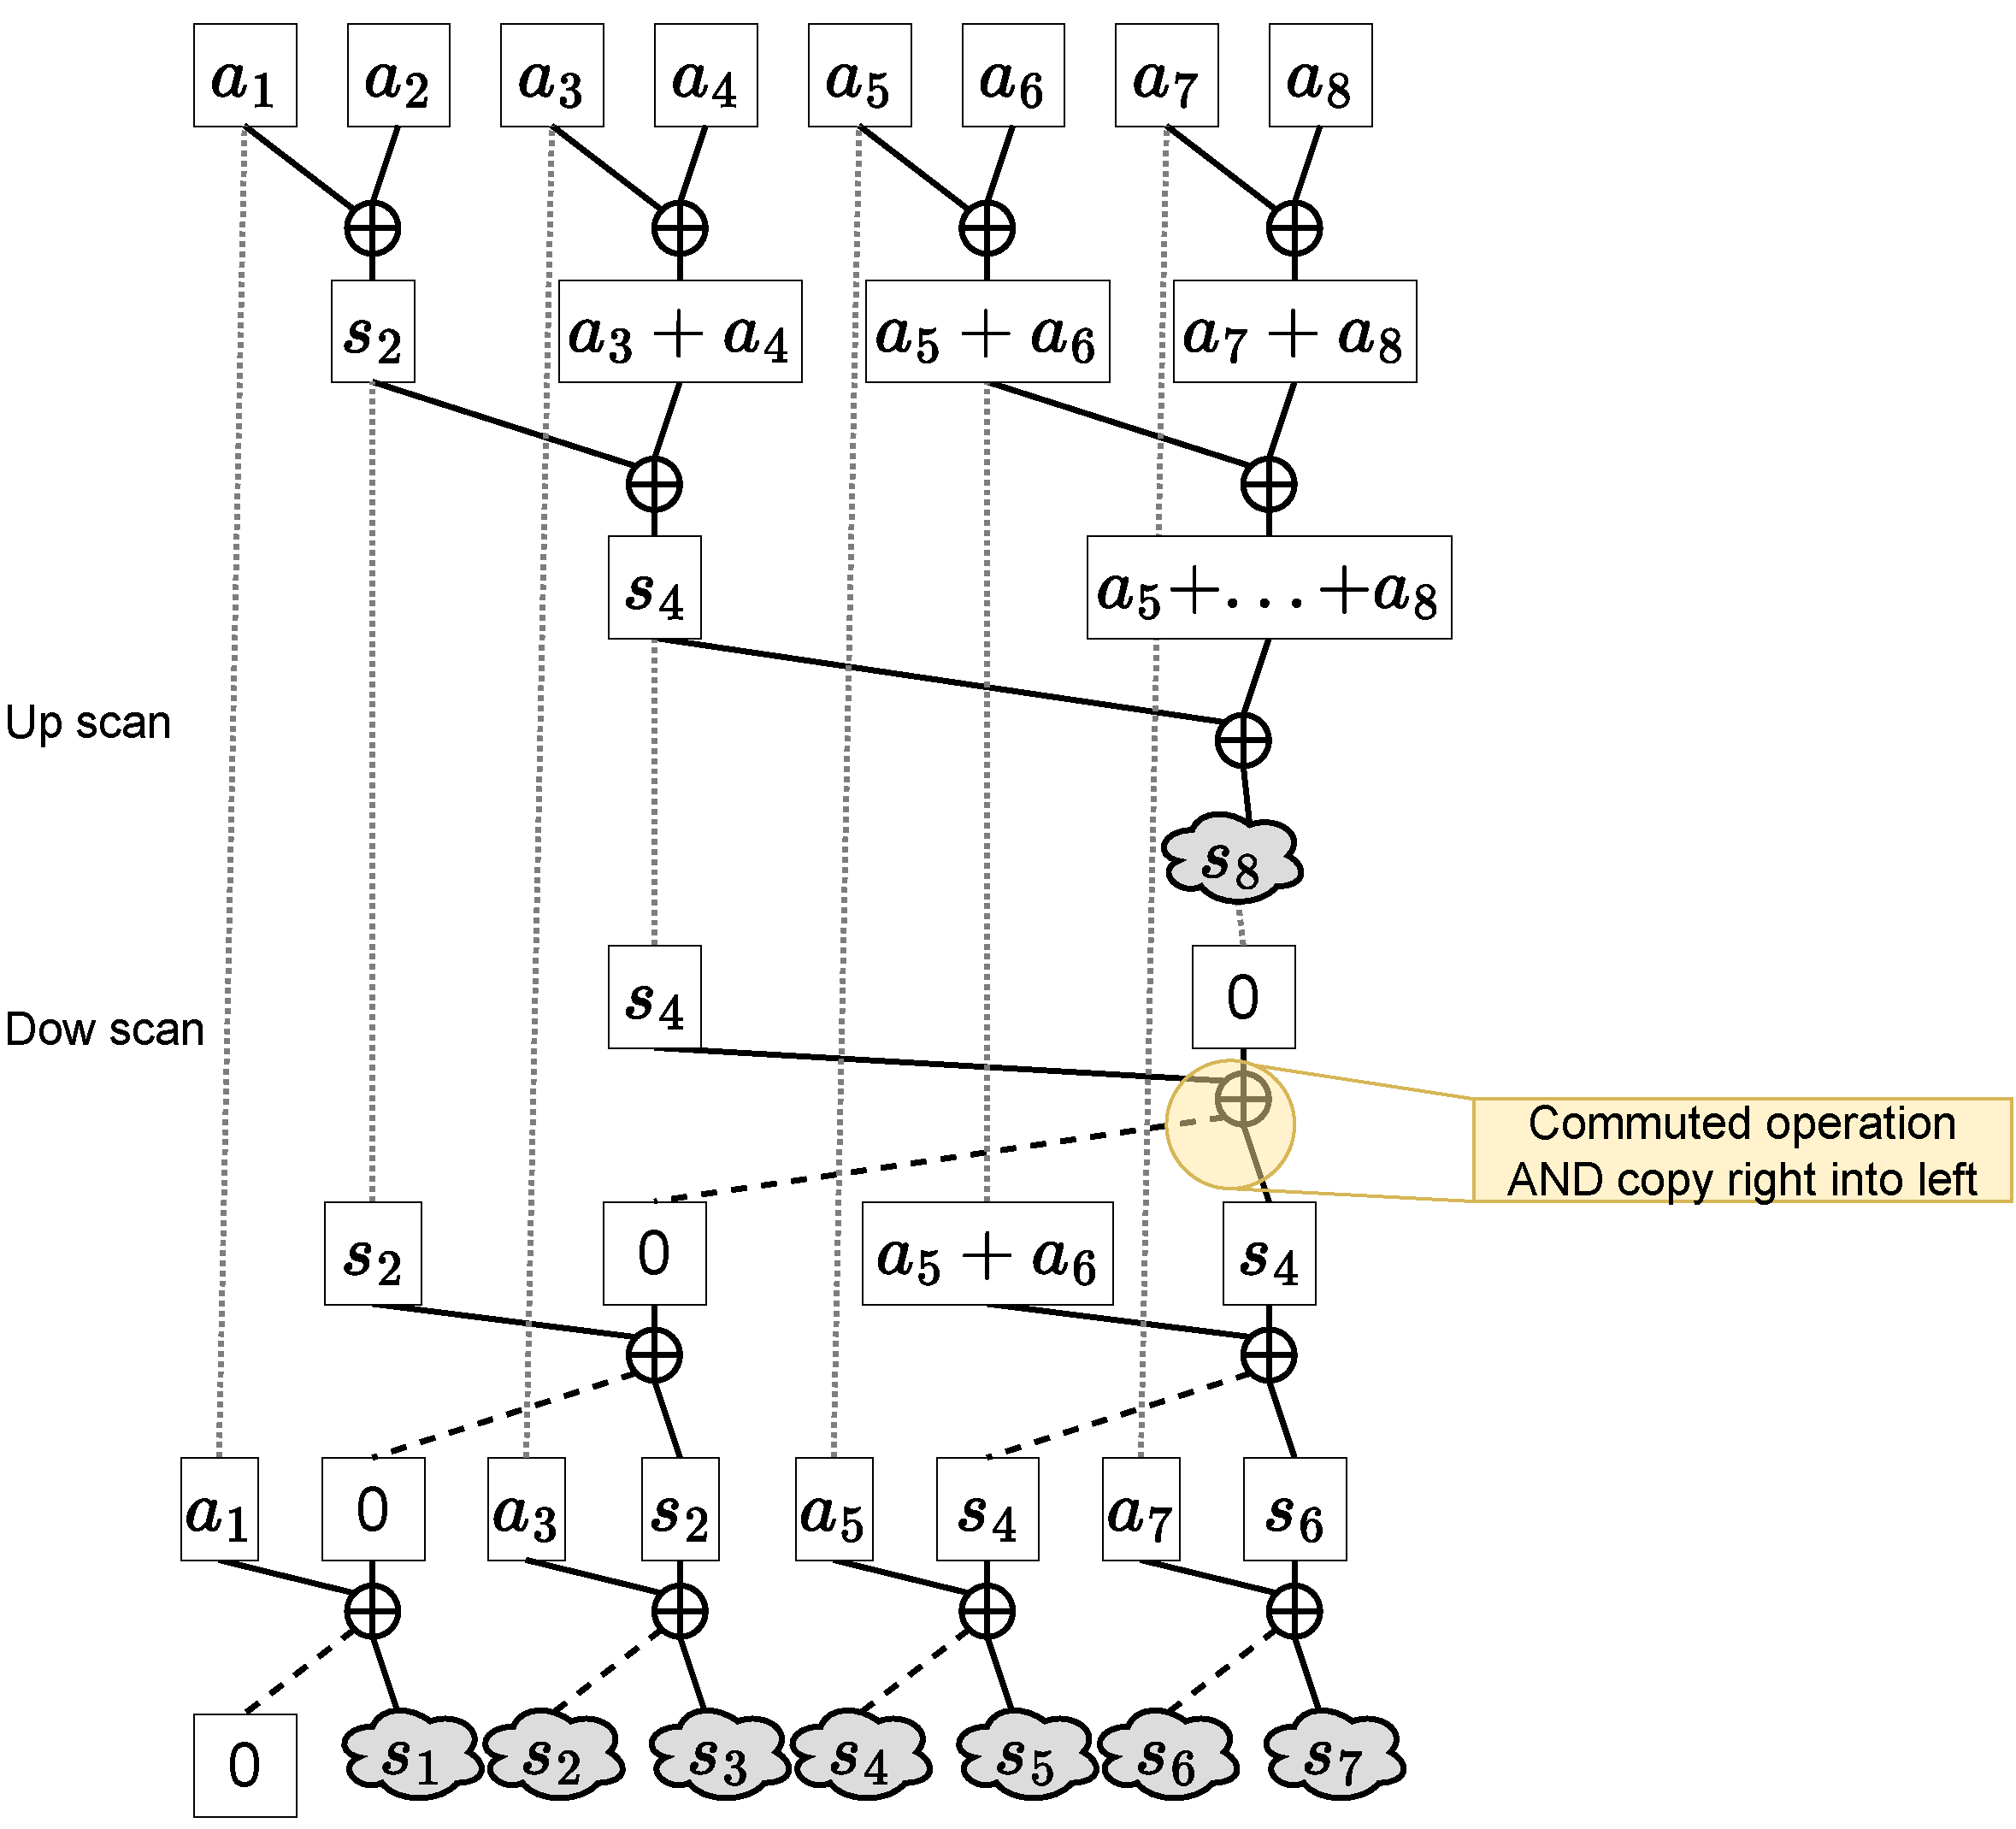
\includegraphics[height=0.3\textheight]{figures/scan_monoid.pdf}
    \hspace{20mm}
    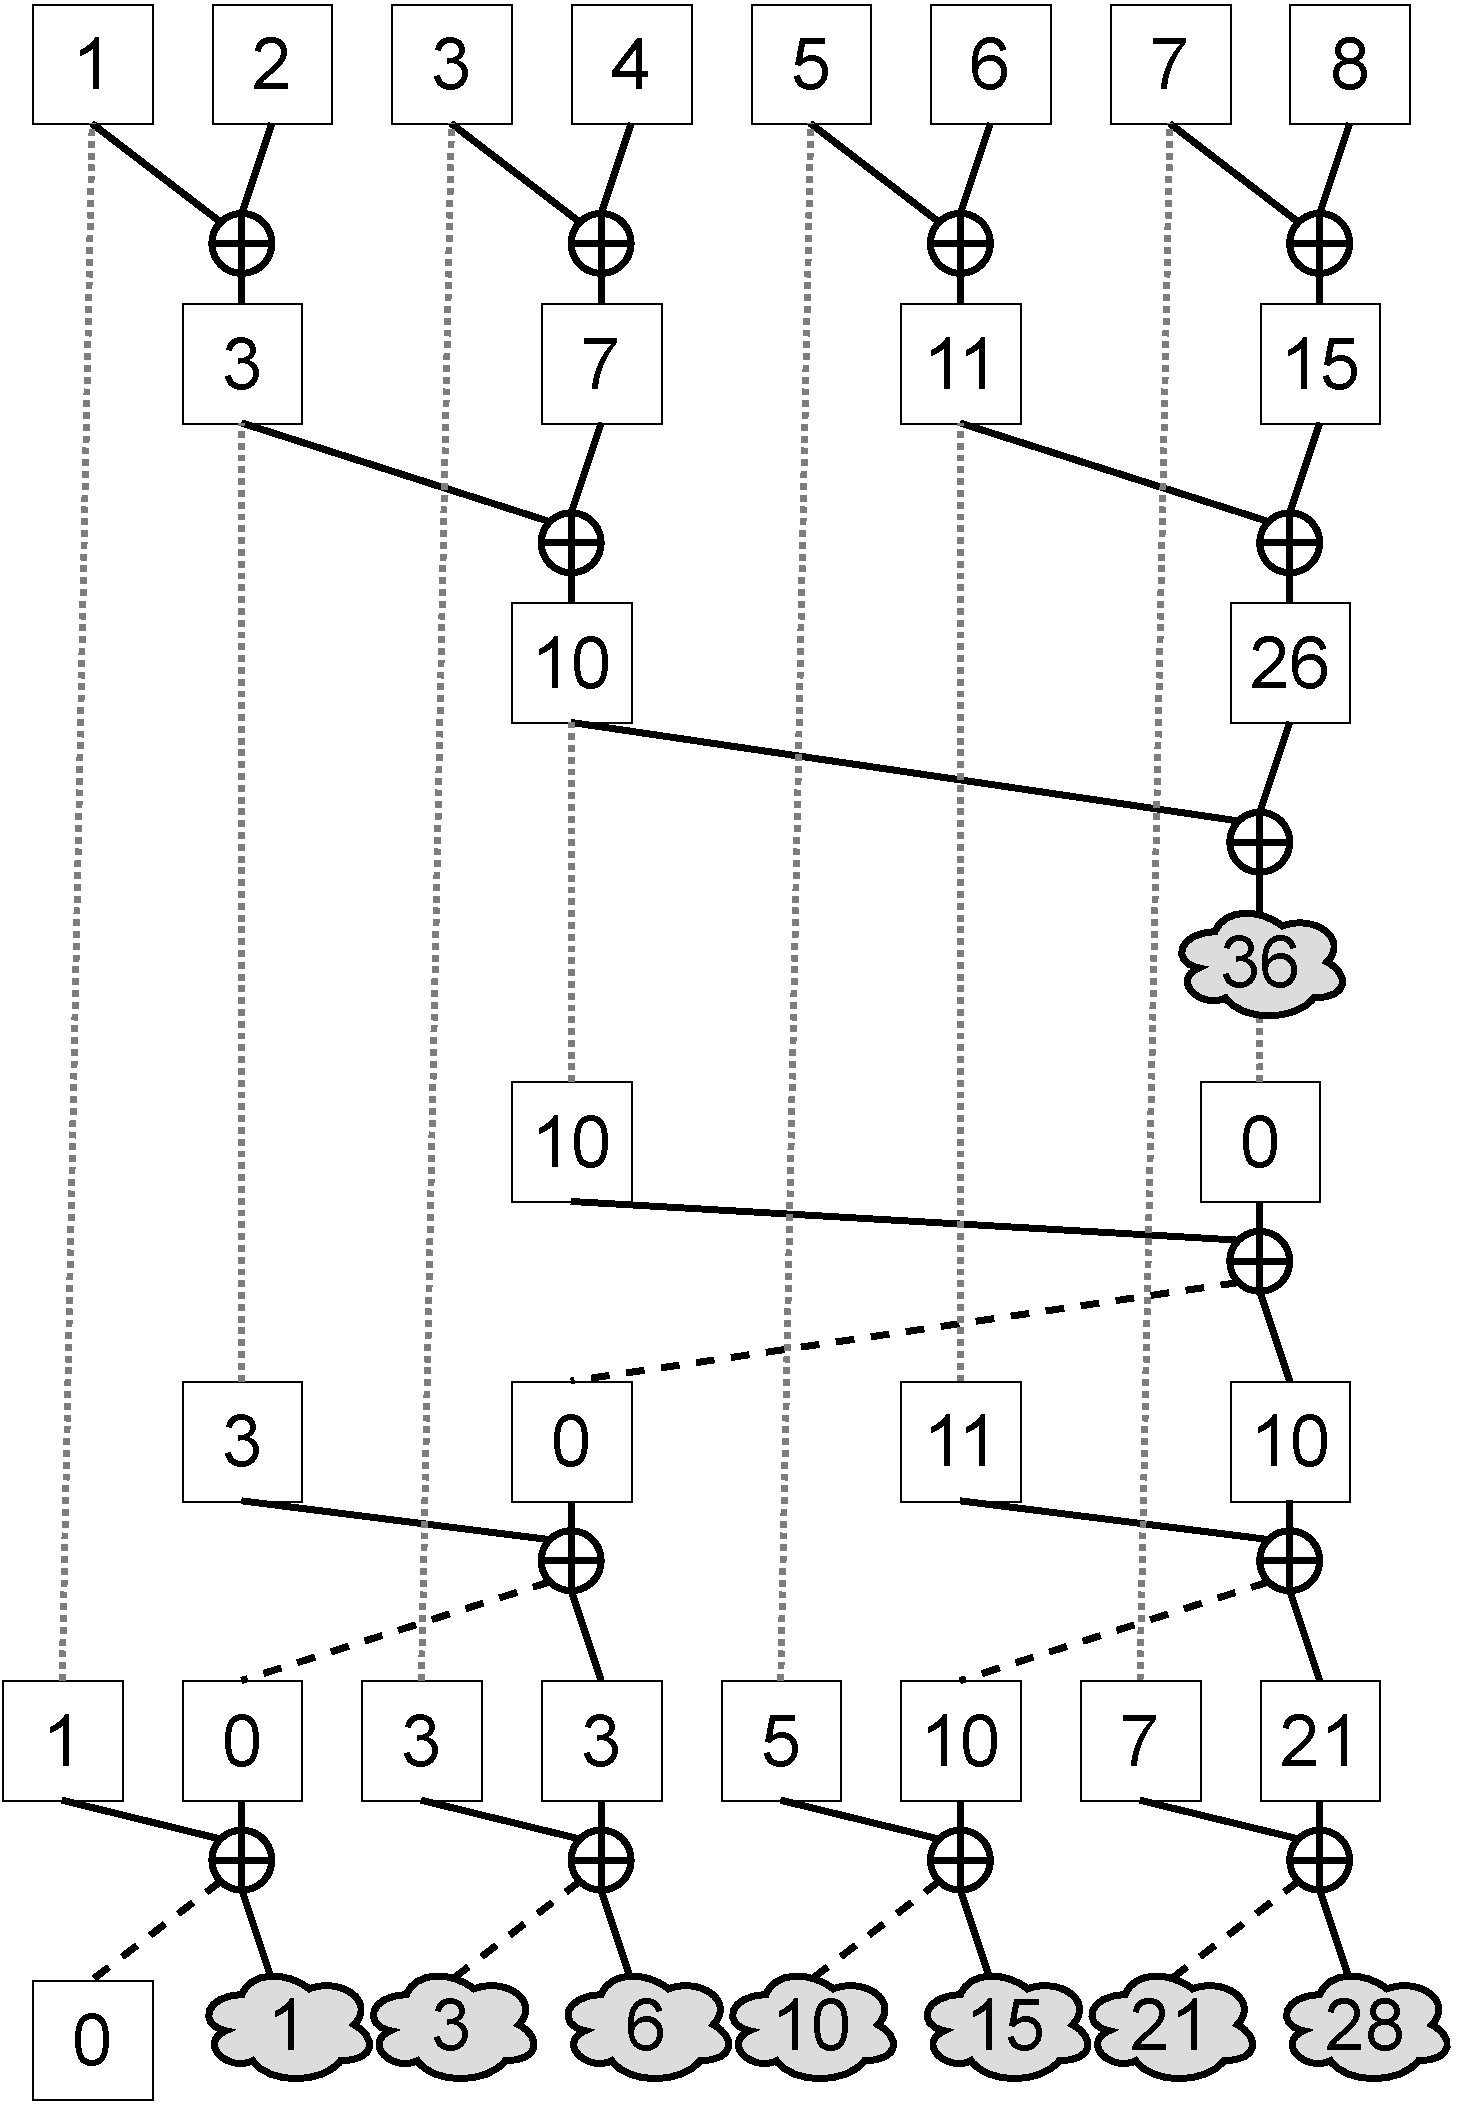
\includegraphics[height=0.3\textheight]{figures/scan_integer.pdf}
    \caption{LEFT: parallel scan with a generic monoid. RIGHT: illustration on the spetial case of natural integers.}
    \label{fig:parallel_scan_general}
\end{figure}

The procedure described above yields $(\sum_{j=0}^{i-1}a_j)_{i\in I}$, with the cumulative sum being $a^{\log_2(T)}_{0}$ the intermediate result of the upward sweep. We analyse the work complexity $W$ and the time complexity $T_\infty$ of $\mathrm{Scan}$ in terms of floating point operations, where $W$ counts the total number of operations needed and $T_\infty$ counts the time complexity under unlimited parallelism.

\begin{ThomasAnnotation}
Note that the output is $\sum_{j=0}^{i-1}a_j$, not $\sum_{j=0}^{i}a_j$ — the scan produces cumulative sums up to but not including the current index (this is the standard definition). The structure of the algorithm (two tree sweeps) is why we get $O(\log T)$ time and $O(T)$ work.
\end{ThomasAnnotation}

\begin{proposition}[Parallel Scan Complexity for $(\N, +)$]
\label{prop:scan_integer_complexity}
    Let $(M, +) \coloneqq (\N, +)$ be the monoid of natural integers equipped with addition. Let $(a_i)_{i\in I}\in \N^I$ be a sequence of integers.

\begin{align}
    W(\mathrm{Scan})&= 2(T-1)\\
    T_\infty(\mathrm{Scan})&= 2\log_2 T
\end{align}
\end{proposition}

\begin{ThomasAnnotation}
These are the headline results for the integer case. The work is $2(T-1)$ because the upward sweep does $T/2 + T/4 + \cdots + 1 = T-1$ operations, and the downward sweep does $1 + 2 + \cdots + T/2 = T-1$ operations. The time is $2\log_2 T$ because there are $\log_2 T$ levels in each sweep, and each level takes 1 unit of time with full parallelism.
\end{ThomasAnnotation}

\begin{proof}
At level $l$ of the upward scan, $U_l = T/(2^{l+1})$ ``$+$'' operations are performed, each of them having a complexity of $1$. There are $\log_2 T$ levels in total. The same goes on for the downward scan, with $D_l = T/(2^{\log_2(T) - l})=2^{l}$ operations at level $l$. Therefore, the work complexity of level $l$ is $U_l$ (resp. $D_l$) while its time complexity is $1$ with unlimited parallelism. It follows that

\begin{align}
\label{eq:W_integer}
W &= 2\sum_{l=0}^{\log_2(T)-1}2^l=2(T-1)\\
\label{eq:T_integer}
T_\infty&= 2\sum_{l=0}^{\log_2(T)-1}1=2\log_2T
\end{align}
\end{proof}

\begin{ThomasAnnotation}
The counting is correct. For the upward sweep: level 0 has $T/2$ operations, level 1 has $T/4$, etc., summing to $T(1/2 + 1/4 + \cdots + 1/T) = T(1 - 1/T) = T-1$. For the downward sweep: level 0 has 1 operation, level 1 has 2, level 2 has 4, etc., up to $T/2$ at the top, summing to $T/2 \cdot (1 + 2 + \cdots) = T/2 \cdot (\text{geometric series})$. Actually, let me recalculate: at level $l$ we have $2^l$ operations, so $\sum_{l=0}^{\log_2(T)-1} 2^l = 2^{\log_2 T} - 1 = T - 1$. Good. The time complexity is simply $\log_2 T$ levels per sweep times 2 sweeps.
\end{ThomasAnnotation}

\subsection{The case of SSM}
\label{sec:scan_SSM}

The case of SSMs is a little more complicated than that of real numbers. In SSMs, the recurrence is defined by \Cref{eq:convssm_recurrence} with the slight modification that kernel convolution is now matrix multiplication and taking $B = I$. Thus, the goal is to compute in parallel the hidden states $(h_i = \sum_{j=0}^i\overline{A}^{i-j}x_j)_i\in I$, where $x_i$ are vectors of dimension $d$ and $\overline{A}$ is a square matrix. This is almost but not quite what we need for the parallel scan. We define the following monoid:

\begin{align}
\label{eq:M_SSM}
    &M^{\mathrm{SSM}}\coloneqq \left\{a = (A, x)\mid A\!\in\!\mathcal{M}_{d}(\R),~x\!\in\!\R^d\right\}\\
\label{eq:+_SSM}
    &(A_a, x_a) +^{\mathrm{SSM}} (A_b,x_b)\coloneqq (A_b \odot A_a, A_b \cdot x_a + x_b)\\
\label{eq:0_SSM}
    &0^{\mathrm{SSM}}\coloneqq(I_d, 0)
\end{align}

\begin{ThomasAnnotation}
The SSM monoid is clever: it pairs a matrix $A$ with a vector $x$. The addition rule is non-commutative: $(A_b, x_b) + (A_a, x_a) = (A_b A_a, A_b x_a + x_b)$ (note the order: $A_b$ multiplies $A_a$ on the left, $A_b$ multiplies $x_a$ then we add $x_b$). This mirrors the structure of SSM unfolding: if you compose two steps of an SSM, the combined transition matrix is the product of the individual ones, and the combined input contribution stacks appropriately.

Wait—I need to check the notation. The definition says $(A_a, x_a) +^{\mathrm{SSM}} (A_b, x_b) \coloneqq (A_b \odot A_a, A_b \cdot x_a + x_b)$. The symbol $\odot$ here means matrix multiplication (confirmed by context, since they later use $\odot$ for element-wise product in spectral). So this is matrix composition: $A_b A_a$.
\end{ThomasAnnotation}

With this monoid structure, and the sequence $(a_i)_{i\in I} \coloneqq ((A, x_i))_{i\in I} \in M^I$, the result of the parallel scan is $((A^i, \sum_{j=0}^iA^{i-j}x_j))_{i\in I}$. The complexity of the scan is less straightforward, but the complexity of each $+^{\mathrm{SSM}}$ operation depends only on $d$, it is a constant of $T$, and therefore, the overall time complexity of the scan is $T_\infty= O(\log T)$ and $W=O(T)$.

\begin{ThomasAnnotation}
Let me verify this claim. If we apply the scan algorithm to the monoid, at each step we combine two pairs $(A, x)$. Let's trace through a small example:
- Input: $((A, x_0), (A, x_1), (A, x_2), (A, x_3))$
- Upward level 0: combine pairs: $(A, x_0) + (A, x_1) = (AA, Ax_0 + x_1)$ and $(A, x_2) + (A, x_3) = (AA, Ax_2 + x_3)$
- Upward level 1: combine: $(AA, Ax_0 + x_1) + (AA, Ax_2 + x_3) = (AAAA, AA(Ax_0 + x_1) + Ax_2 + x_3) = (A^4, A^3 x_0 + A^2 x_1 + A x_2 + x_3)$

For $i=3$, the result should be $\sum_{j=0}^{3} A^{3-j} x_j = A^3 x_0 + A^2 x_1 + A x_2 + x_3$. Yes, this matches! So the monoid is correct and associative. The identity is $(I_d, 0)$ because $(A, x) + (I_d, 0) = (A, Ax + 0) = (A, Ax)$... wait, that doesn't work. Let me check the identity. If we want $(A, x) + (I, 0) = (A, x)$, then we need $I \odot A = A$ and $I \cdot x + 0 = x$. This works if $I$ is the identity matrix.

Hmm, but actually I need to check whether the operation is truly associative. Let me verify:
- $(a + b) + c$ vs. $a + (b + c)$ where $a = (A_a, x_a)$, $b = (A_b, x_b)$, $c = (A_c, x_c)$.
- $(a + b) + c = (A_b A_a, A_b x_a + x_b) + (A_c, x_c) = (A_c(A_b A_a), A_c(A_b x_a + x_b) + x_c) = (A_c A_b A_a, A_c A_b x_a + A_c x_b + x_c)$
- $a + (b + c) = (A_a, x_a) + (A_c A_b, A_c x_b + x_c) = (A_c A_b A_a, A_c A_b x_a + A_c x_b + x_c)$

Great, they match! So associativity holds.
\end{ThomasAnnotation}

\begin{proposition}[SSM Complexity]
\label{prop:SSM_complexity}
    Let $(M, +) \coloneqq (M^{\mathrm{SSM}}, +^{\mathrm{SSM}})$ be the monoid defined by \Cref{eq:M_SSM,eq:+_SSM,eq:0_SSM}. Let $(a_i)_{i\in I}\in (M^{\mathrm{SSM}})^I$.

\begin{align}
    W(\mathrm{Scan})&= 2(T-1)(d^3+d^2+d)\\
    T_\infty(\mathrm{Scan})&= 2\log_2 (T) (d^3+d^2+d)
\end{align}
\end{proposition}

\begin{ThomasAnnotation}
The key insight: each $+^{\mathrm{SSM}}$ operation involves (1) matrix-matrix multiplication $A_b A_a$ costing $O(d^3)$, (2) matrix-vector multiplication $A_b x_a$ costing $O(d^2)$, and (3) vector addition costing $O(d)$. Since there are $2(T-1)$ operations in total (from integer case), the total work is $2(T-1) \times (d^3 + d^2 + d)$. The time is $2 \log_2 T$ levels (from integer case) times $(d^3 + d^2 + d)$ per operation.
\end{ThomasAnnotation}

\begin{proof}
The proof of \Cref{prop:scan_integer_complexity} applies with the only difference that now, each $+^{\mathrm{SSM}}$ operation has complexity $d^3$ for the matrix multiplication on the left, $d^2$ for the matrix-vector multiplication and $d$ for the vector addition on the right.
\end{proof}

\begin{ThomasAnnotation}
This is correct, but the proof glosses over the fact that we're now applying the integer-case structure with a different cost per operation. The structure of the algorithm (number and nesting of operations) stays the same; only the cost changes.
\end{ThomasAnnotation}

\subsection{The problem of convolution}
\label{sec:spatial_ConvSSM}

Moving from $d$ dimensional vectors to images with $c$ channels and $h \times w$ spatial dimension and from matrix multiplication to spatial convolution, we can rewrite our monoid structure as :
\begin{align}
    &M^{\mathrm{Conv}_1}\coloneqq \left\{a = (K, I)\mid \exists k_1, k_2,\quad K\!\in\!\R^{k_1\times k_2\times c\times c},~I\!\in\!\R^{h \times w \times c}\right\}\\
    &(K_a, I_a) +^{\mathrm{Conv}_1} (K_b,I_b)\coloneqq (K_b \circledast K_a, K_b \ast I_a + I_b)\\
    &0\coloneqq(I, 0)
\end{align}

\begin{ThomasAnnotation}
The spatial ConvSSM monoid extends the SSM monoid by replacing vectors with spatial feature maps and matrices with spatial kernels. The addition now involves kernel-kernel convolution (denoted $\circledast$) and kernel-feature convolution (denoted $\ast$). The notation is: $K$ is a 4D tensor (kernel height $\times$ width $\times$ input channels $\times$ output channels), and $I$ is a 3D feature map (height $\times$ width $\times$ channels).
\end{ThomasAnnotation}

\noindent where $\circledast$ is the convolution between two kernels and $\ast$ is the convolution between a kernel and an image:

\begin{align*}
    & \forall \left\{
\begin{aligned}
    &x\!\in\!\intint{0}{h\!-\!1}\\
    &y\!\in\!\intint{0}{w\!-\!1}\\
    &c_{\mathrm{out}}\!\in\!\intint{1}{c}
\end{aligned}
\right., (K\!\ast\!I)_{x,y,c_{\mathrm{out}}} = \sum_{u=0}^{k_1-1}\sum_{v=0}^{k_2-1}\sum_{i=1}^{c} K_{u,v,i,c_{\mathrm{out}}} I_{(x-u,y-v)\%(h,w),i}\\
    & \forall \left\{
\begin{aligned}
    &u\!\in\!\intint{0}{k_1\!+\!l_1\!-\!2}\\
    &v\!\in\!\intint{0}{k_2\!+\!l_2\!-\!2}\\
    &c_{\mathrm{in}},c_{\mathrm{out}}\!\in\!\intint{1}{c}
\end{aligned}
\right., (L \circledast K)_{u,v,c_{\mathrm{in}},c_{\mathrm{out}}} = \sum_{p=0}^{l_1-1}\sum_{q=0}^{l_2-1}\sum_{c_{k}=1}^{c} L_{p,q,c_{k},c_{\mathrm{out}}} K_{u-p,v-q,c_{\mathrm{in}},c_{k}}\text{, $K$ being zero-padded}\\\end{align*}

\noindent with $L\!\in\!\R^{l_1\times l_2\times c \times c}$, $K\!\in\!\R^{k_1\times k_2\times c \times c}$ and $I\!\in\!\R^{h \times w \times c}$

\begin{ThomasAnnotation}
The kernel-feature convolution $(K \ast I)$ is the standard CNN convolution: for each output position $(x, y)$ and channel $c_{\mathrm{out}}$, we slide the kernel and compute a weighted sum over the input. The modulo arithmetic $\%(h, w)$ indicates circular/toroidal boundary handling.

The kernel-kernel convolution $(L \circledast K)$ is trickier: it convolves two kernels. The output kernel size is $(l_1 + k_1 - 1) \times (l_2 + k_2 - 1)$, which is the key problem: kernel sizes grow!
\end{ThomasAnnotation}

With this structure, the key aspect is that the spatial size of the kernel resulting from $\circledast$ is the sum of the sizes of the input kernels. Therefore, the parallel scan algorithm operates on larger and larger kernel sizes, with sizes growing exponentially with the depth in the tree structure. The complexity of our $+$ operator is thus no more constant as it depends on the depth. The bottleneck is at the very last layer of the upward scan, where kernel size is $O(Tk)$, with $k$ the size of the original kernel $K$, resulting in a single $\ast$ operation whose complexity is in $O(T^2)$. This bottleneck is illustrated in \Cref{fig:parallel_scan_conv_spatial}.

\begin{ThomasAnnotation}
This is the core problem. At each level $l$ of the upward scan, the kernel size grows from the original $k \times k$ to approximately $(2^{l+1} - 1) k \times (2^{l+1} - 1) k$ (due to repeated convolution). By the top level, kernel size is $O(T) \times O(T)$, so a single convolution operation with that kernel costs $O(T^2)$. Since there's only one such operation (at the very top), the work is $O(T^2)$ in the worst case.
\end{ThomasAnnotation}

\begin{proposition}[Spatial ConvSSM Complexity]
    Let $(M, +) \coloneqq (M^{\mathrm{Conv}_1}, +^{\mathrm{Conv}_1})$ be the monoid defined by \Cref{eq:M_SSM,eq:+_SSM,eq:0_SSM}. Let $(a_i)_{i\in I}\in (M^{\mathrm{Conv}_1})^I$.

\begin{align}
    W&= O(T^2)\\
    T_\infty&= O(W)
\end{align}
\end{proposition}

\begin{ThomasAnnotation}
The time complexity $T_\infty = O(W)$ means there is essentially no parallelism benefit: all operations happen sequentially. This is because the bottleneck operation (the final convolution with the large kernel) dominates and cannot be parallelized.
\end{ThomasAnnotation}

\begin{proof}
The proof of \Cref{prop:scan_integer_complexity} applies with the major difference that on the upward scan, at level $l$, each $+^{\mathrm{Conv}_1}$ operation has complexity $(k+(2^l-1)(k-1))\times (k+(2^l-1)(k-1))\times c^3 = O((2^l)^2\times k^2 \times c^3)$ for the kernel-kernel convolution on the left, $O(h \times w \times (2^l)^2\times k^2 \times c^2)$ for the kernel-image convolution and $h \times w\times c$ for the image addition on the right. The same goes on for the downward scan.

\begin{ThomasAnnotation}
Let me parse the kernel size formula. At level 0, kernel is $k \times k$. At level 1, we convolve two $k \times k$ kernels, yielding $(k + k - 1) \times (k + k - 1) = (2k - 1) \times (2k - 1)$. At level 2, we convolve a $(2k-1) \times (2k-1)$ kernel with another, yielding $(2k - 1 + k - 1) \times \cdots = (3k - 2) \times (3k - 2)$. In general, at level $l$, the kernel is approximately $(2^{l+1} - 1)(k - 1) + 1 \approx 2^{l+1} k$ in size (for large $k$). Wait, let me recount: $(k + (2^l - 1)(k - 1)) = k + 2^l k - 2^l - k + 1 = 2^l k - 2^l + 1 = (2^l)(k-1) + 1$. Hmm, the formula in the proof is a bit different. Let me just trust it for now and note that it's roughly $O((2^l)^2 \times k^2)$ in operation count.

For the kernel-kernel convolution, the operation count is the product of kernel sizes, which is $(kernel\_size)^2 \times c^{\text{in}} \times c^{\text{out}} = O((2^l)^2 k^2 c^3)$ (since we're iterating over all spatial positions and all input/output channel pairs).

For the kernel-image convolution, the operation count is $h \times w$ spatial positions times the kernel size squared times the channel operations: $h \times w \times (2^l)^2 k^2 \times c^2$.
\end{ThomasAnnotation}

Thus, \Cref{eq:W_integer,eq:T_integer} become :

\begin{align}
\label{eq:W_conv}
W &= O(2 \sum_{l=0}^{\log_2(T)-1} 2^{\log_2(T)-(l+1)} \times \left[ (2^l)^2\times k^2 \times c^3 + h \times w \times (2^l)^2\times k^2 \times c^2\right])\\
&= O(T^2 \times k^2 \times c^3) + O(T^2 \times h \times w \times k^2 \times c^2)\\
\label{eq:T_conv}
T_\infty&= O(2\sum_{l=0}^{\log_2(T)-1} \left[ (2^l)^2\times k^2 \times c^3 + h \times w \times (2^l)^2\times k^2 \times c^2\right])\\
&= O(W)
\end{align}
\end{proof}

\begin{ThomasAnnotation}
The first equation sums over all levels of both sweeps. At level $l$, there are $2^{\log_2(T) - (l+1)} = T / 2^{l+1}$ operations in the upward sweep, each costing $O((2^l)^2 k^2 c^3)$. Summing over $l$ gives:
$$\sum_{l=0}^{\log_2(T)-1} \frac{T}{2^{l+1}} \times (2^l)^2 k^2 c^3 = T k^2 c^3 \sum_{l=0}^{\log_2(T)-1} \frac{2^l}{2} = \frac{T k^2 c^3}{2} (T - 1) \approx O(T^2 k^2 c^3)$$

Similarly for the kernel-image term, giving $O(T^2 h w k^2 c^2)$. The downward sweep contributes the same order of magnitude. So the claim $W = O(T^2 k^2 c^3)$ is correct.

For $T_\infty$, the sum is now over the time per level (not the number of operations per level), so we're summing the maximum operation complexity at each level:
$$T_\infty = 2 \sum_{l=0}^{\log_2(T)-1} O((2^l)^2 k^2 c^3) = O(2 \sum_{l=0}^{\log_2(T)-1} (2^l)^2 k^2 c^3)$$

The $\sum_{l=0}^{\log_2(T)-1} (2^l)^2 = \sum_{l=0}^{\log_2(T)-1} 4^l = \frac{4^{\log_2(T)} - 1}{3} = \frac{T^2 - 1}{3} = O(T^2)$. So $T_\infty = O(T^2 k^2 c^3) = O(W)$, confirming the claim.
\end{ThomasAnnotation}

\begin{figure}[ht]
    \centering
    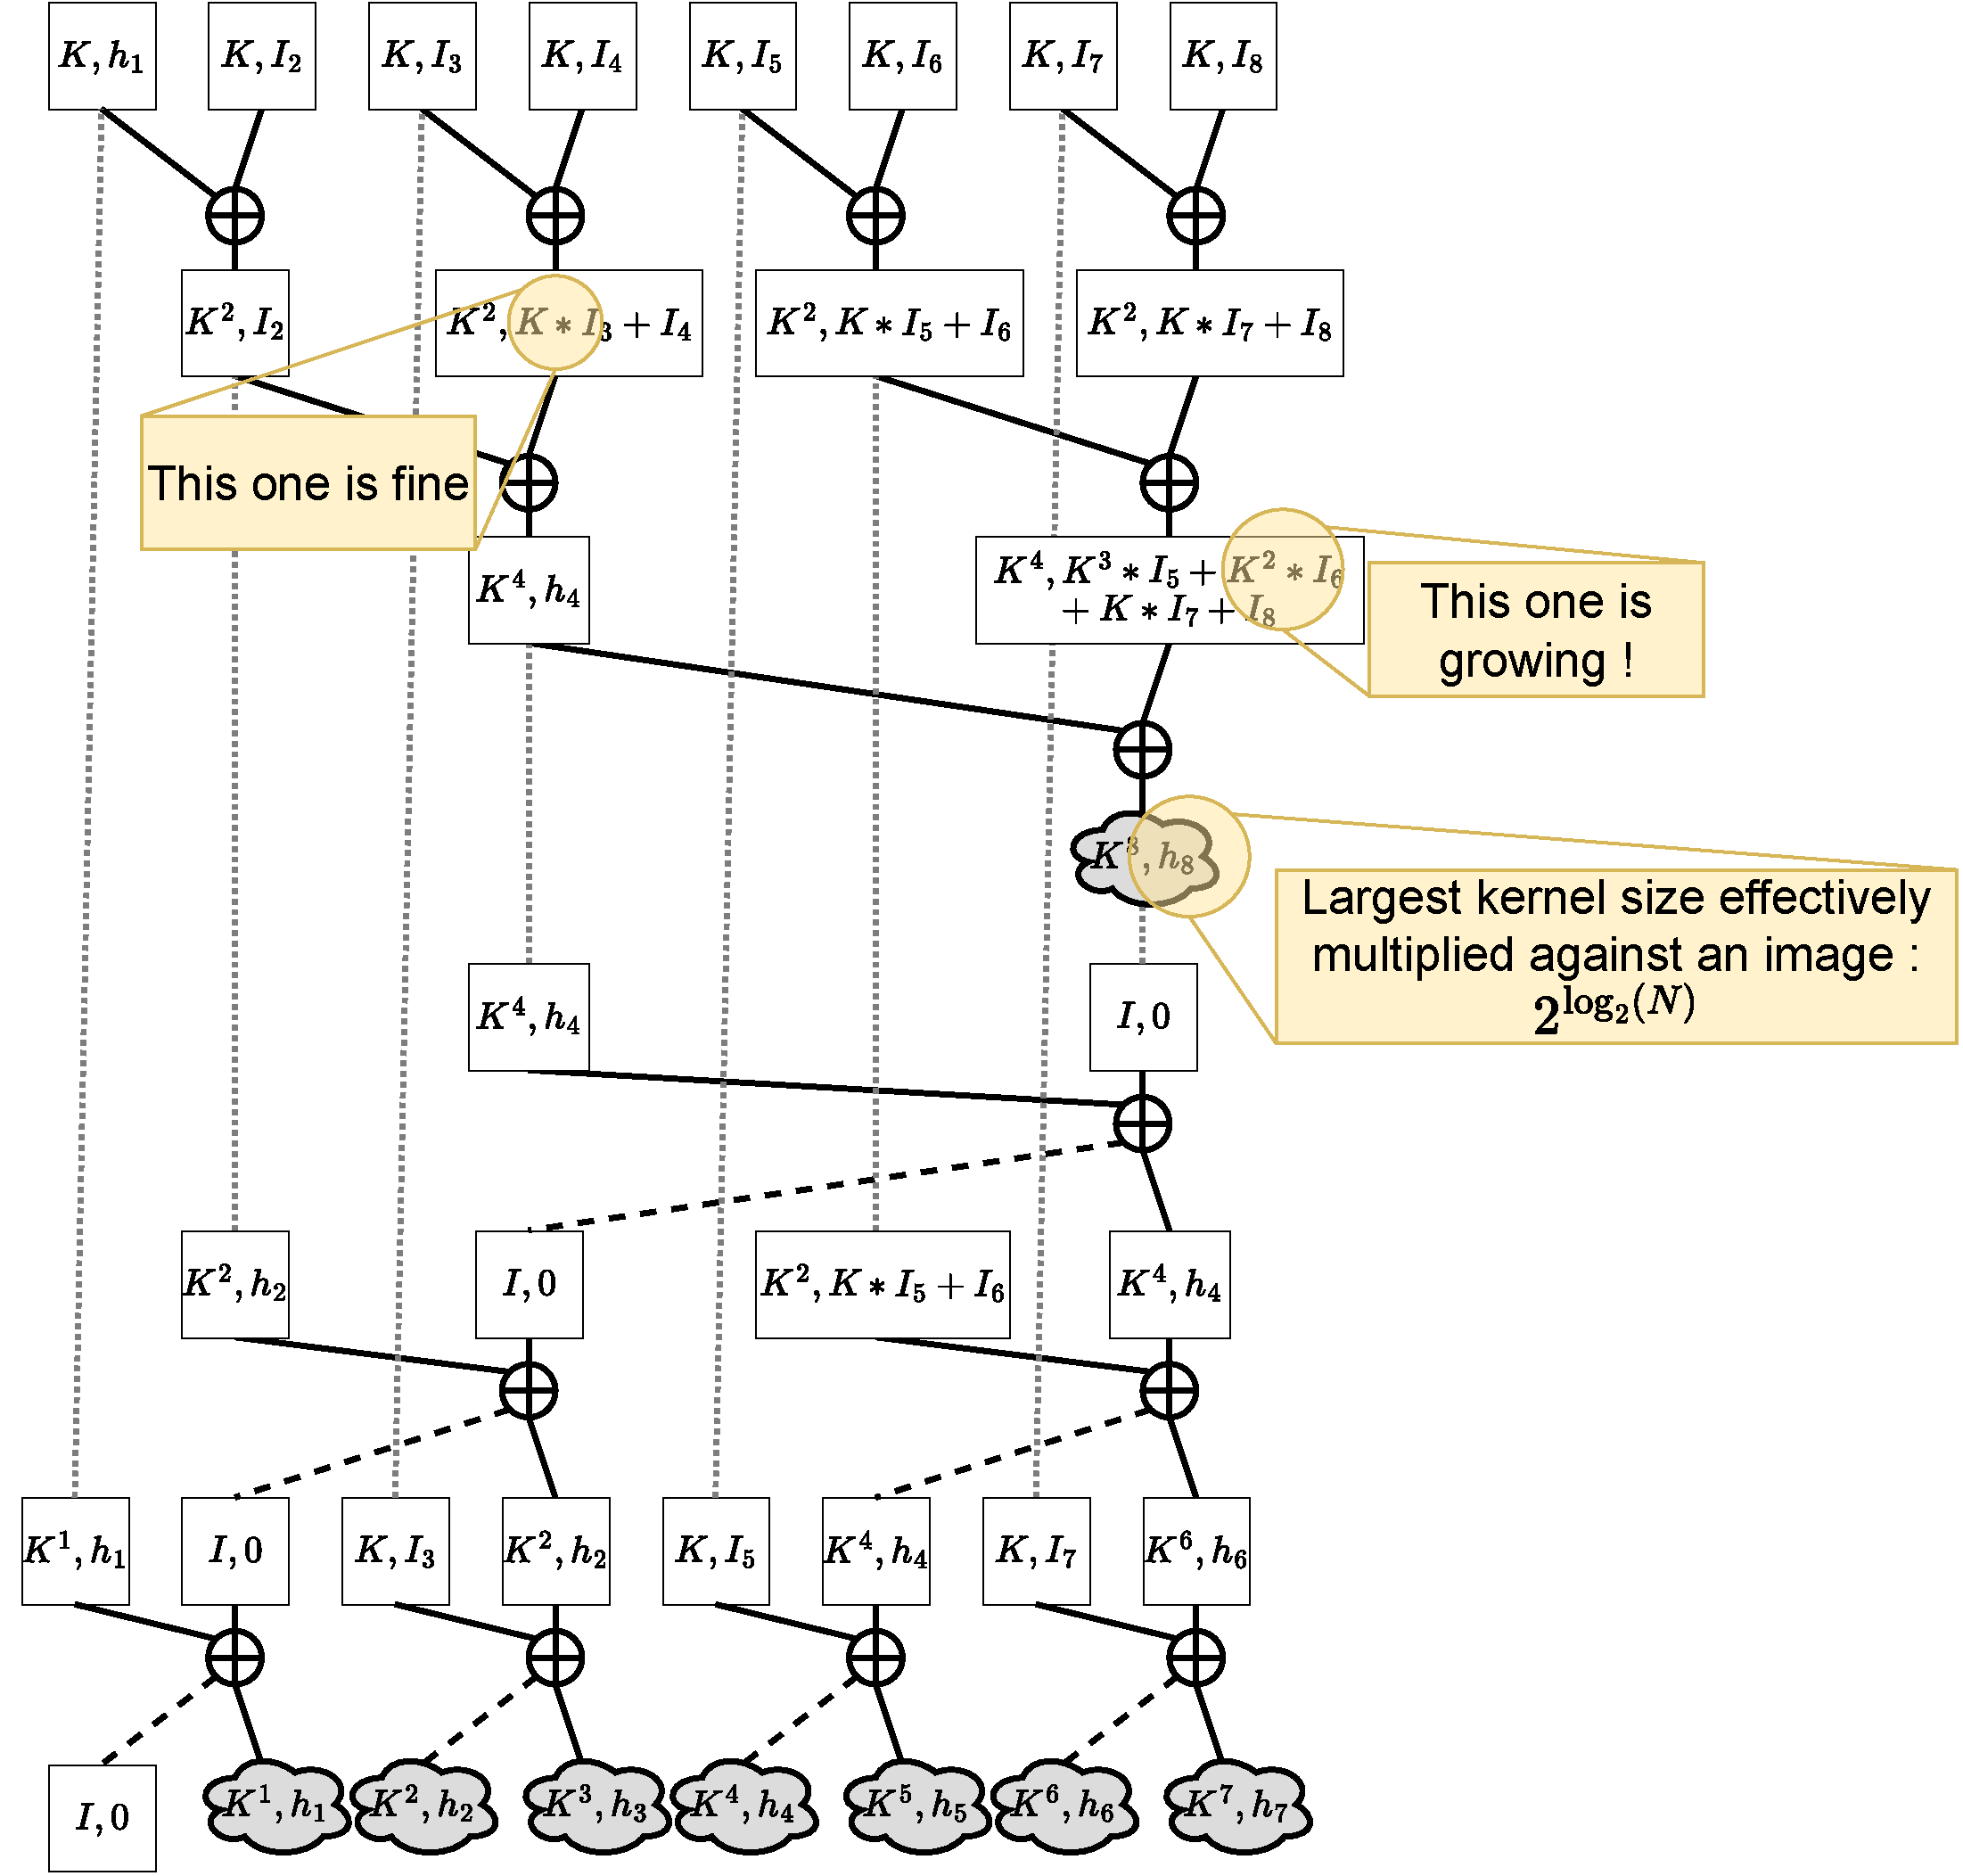
\includegraphics[height=0.3\textheight]{figures/scan_conv.pdf}
    \caption{Parallel scan applied to the monoid structure defined for spatial convolution SSM. Highlighted is the core of the issue : growing kernels lead to a bottleneck where a single operation has $O(T^2)$ complexity.}
    \label{fig:parallel_scan_conv_spatial}
\end{figure}

\subsection{How spectral domain solves the issue}
\label{sec:spectral_ConvSSM}

To dispell the curse of growing kernels we move to the spectral domain. In this domain, our monoid becomes:
\begin{align}
\label{eq:M_SSM_spectral}
    &M^{\mathrm{Conv}_2}\coloneqq \left\{ a = (\hat{K}, \hat{I})\,\middle|\,\exists (K, I)\in M^{\mathrm{Conv}_1},\Bigl\{\begin{aligned}
    &\hat{K} = \mathrm{FFT}(K_{\mathrm{padded}})\in \C^{h\times w\times c\times c}\\
    &\hat{I} = \mathrm{FFT}(I)\in \C^{h\times w\times c}
\end{aligned}
\Bigr.\right\}\\
\label{eq:+_SSM_spectral}
    &(\hat{K}_a, \hat{I}_a) +^{\mathrm{Conv}_2} (\hat{K}_b,\hat{I}_b)\coloneqq (\hat{K}_b \odot \hat{K}_a, \hat{K}_b \cdot \hat{I}_a + \hat{I}_b)\\
\label{eq:0_SSM_spectral}
    &0\coloneqq(I, 0)
\end{align}

\begin{ThomasAnnotation}
This is the key insight: by moving to the Fourier domain, spatial convolution becomes element-wise multiplication. The kernels and images are now represented as their FFTs (complex-valued tensors of size $h \times w \times c \times c$ and $h \times w \times c$ respectively). The symbol $\odot$ now means element-wise matrix multiplication (not matrix multiplication as before).

Critically, in the spectral domain, the "kernel" at each frequency bin has fixed size $h \times w$, so there's no kernel growth. The operations $\hat{K}_b \odot \hat{K}_a$ and $\hat{K}_b \cdot \hat{I}_a$ now take constant time per frequency bin.
\end{ThomasAnnotation}

\noindent with $\odot$ the element-wise matrix multiplication and $\cdot$ the element-wise matrix-vector multiplication. With this operator, the kernel grows no more, the cost is again a constant of time and depth, depending only on $h$, $w$ and $c$. We are thus back to a time complexity for the parallel scan of $O(\log T)$.

\begin{ThomasAnnotation}
The statement "element-wise matrix multiplication" means: for each frequency bin $(w_1, w_2)$, we have matrices $\hat{K}_{a, w_1, w_2} \in \C^{c \times c}$ and $\hat{K}_{b, w_1, w_2} \in \C^{c \times c}$, and we compute their matrix product independently at each frequency. The total work is thus $O(h \times w \times c^3)$ (since we do $h \times w$ matrix multiplications of size $c \times c$ each).
\end{ThomasAnnotation}

\begin{proposition}[Spectral ConvSSM Complexity]
\label{prop:spectral_conv_complexity}
    Let $(M, +) \coloneqq (M^{\mathrm{Conv}_2}, +^{\mathrm{Conv}_2})$ be the monoid defined by \Cref{eq:M_SSM_spectral,eq:+_SSM_spectral,eq:0_SSM_spectral}. Let $(a_i)_{i\in I}\in (M^{\mathrm{Conv}_2})^I$.

\begin{align}
    W&= O(T)\\
    T_\infty&= O(\log_2T)
\end{align}
\end{proposition}

\begin{ThomasAnnotation}
Excellent: we're back to the same complexity as the standard SSM case (Proposition~\ref{prop:SSM_complexity}), with the constant depending on image size ($h \times w$) and channels ($c$), not on sequence length ($T$). This is the main result.
\end{ThomasAnnotation}

\begin{proof}
The proof of \Cref{prop:scan_integer_complexity} applies with the only difference that now, each $+^{\mathrm{Conv}_2}$ operation has complexity $h \times w \times c^3$ for the kernel-kernel multiplication on the left, $h \times w \times c^2$ for the kernel-image multiplication and $h \times w \times c$ for the image addition on the right. This gives :

\begin{align}
\label{eq:W_spectral}
    W&= O(T \times h \times w \times c^3)\\
\label{eq:T_spectral}
    T_\infty&= O(\log_2T \times h \times w \times c^3)
\end{align}
\end{proof}

\begin{ThomasAnnotation}
Each $+^{\mathrm{Conv}_2}$ operation involves:
1. Element-wise matrix multiplication at $h \times w$ frequency bins, each costing $c^3$ (matrix multiply of $c \times c$ matrices).
2. Element-wise matrix-vector multiplication at $h \times w$ frequency bins, each costing $c^2$.
3. Element-wise vector addition at $h \times w$ frequency bins, each costing $c$.

Total: $h \times w \times (c^3 + c^2 + c)$. Since there are $O(T)$ operations in the scan (from the integer case), we get $W = O(T \times h \times w \times c^3)$. The time is $O(\log_2 T \times h \times w \times c^3)$.

One critical detail: does the equivalence between spatial convolution and element-wise multiplication in the Fourier domain actually hold? Yes, by the convolution theorem: if $y = K \ast I$ in spatial domain, then $\hat{y} = \hat{K} \odot \hat{I}$ in frequency domain (where $\odot$ is element-wise multiplication). So this is mathematically sound.
\end{ThomasAnnotation}

% \section{Recurrence kernel parameterisation}

% TODO : capability subsection vs complexity subsection vs optimisation subsection

% capability :
% - log domain : multiplicative dynamics in log domain match biological divisive norms. Write it up properly : K*I + I in spatial or spectral is linear, but K*I + I in cepstral becomes K*I * I in spectral - this is the multiplicative dynamic.
% - scale equivariance through wavelets
% - diagoanlisable vs non diagonalisable comment : tradeoff between complexity (cref(sec:TODO below)) and expressivity.
% - anything else ?

% complexity :
% - log domain : This preserves the complexity analysis of section \cref{sec:spectral_ConvSSM}, as you only need to change $+^{\mathrm{Conv}_2}$ such that the right hand side multiplies element wise the images instead of adding them. Then we can operate in log domain.
% - in the fourier space K*K is in $c^3$, and K*I is in $c^2$ (\cref{eq:W_spectral,eq:T_spectral}) : if every frequency bin is diagonalisable, NPLR (normal plus low rank) or something, then this cost can be cut down to $c$ for both. Question : how to actually parameterise spatial domain to have this spectral property ? Would it be easier to parameterise in fourier with constraints such that the spatial domain of the kernel is still k*k ?
% - anything else ?

% optimisation :
% - log domain : It makes BPTT much easier as exponential behaviors mess up gradients but in log domain it is linear
% - orthogonal convolution : this also controls exponential behavior through eigenvalues of 1, but it comes at the cost of expressivity and doesn't have the divisive behavior in log domain. Maybe combine both log domain and orthogonal convolution ? though with log domain you already have what orthogonal brings to the table so maybe it's a bad idea and you just lose expressivity..
% - anything else ?

\subsection{Taking down the constant}
\label{sec:the_constant}

Now that we have solved the main issue of complexity explosion with time, we tackle the problem of the constant. As mentioned in \Cref{prop:SSM_complexity}, as is, the work complexity is $O(T)$ with a constant that is $O(d^3)$ due to matrix multiplications.

\begin{ThomasAnnotation}
The problem: even though $W = O(T)$ for spectral ConvSSM, the constant $h \times w \times c^3$ can be large. For a $256 \times 256$ image with $512$ channels, $h \times w \times c^3 = 256^2 \times 512^3$ is prohibitive. The goal is to reduce the $c^3$ factor.
\end{ThomasAnnotation}

\citet{TODO:S4SSM} proposed to reparameterise the recurrence matrix $A$ to be normal plus low rank (NPLR) in order to reduce this constant from $O(d^3)$ to $O(d)$. The complexity gain comes from the change of basis being absorbed outside of the recurrence such that the recurrence can operate on diagonalized matrices. Note that their approach to parallelization through time uses the convolution view of the SSM, not the parallel scan as proposed by \citet{TODO:S5SSM}.

\begin{ThomasAnnotation}
The idea: if $A$ can be diagonalized, then $A = V D V^{-1}$ where $D$ is diagonal. Computing $A^k$ becomes $V D^k V^{-1}$, where $D^k$ is cheap (just raising diagonal entries to the $k$-th power). But not all matrices are diagonalizable. The NPLR trick is to write $A = \Lambda + P Q^\top$ where $\Lambda$ is a diagonal part and $PQ^\top$ is a low-rank part. By carefully choosing the change of basis, you can work in a basis where the recurrence is cheap.
\end{ThomasAnnotation}

In our case, this $O(c^3)$ is even more prohibitive as it is repeated over each pixel position, with the total constant being $O(k^2c^3 + hwk^2c^2)$ in the spatial domain, and $O(hwc^3)$ in the spectral domain.

In spatial domain, this parameterization translates to having a shared change of basis $V$ for each $K_{x,y}$. This way, $V$ can be factored our ot the kernel such that the resulting kernel follows~: $\forall x,y, \mathcal{K}_{x,y} = \Lambda_{x,y} + P_{x,y} Q_{x,y}^\top$, where
\begin{itemize}
    \item $\Lambda_{x,y}$ are block diagonal with blocks of rank at most $2$ in real domain, and diagonal with eigenvalues of modulus 1 in complex domain. With the complex view, $\mathcal{K}$ is diagonal plus low rank (DPLR).
    \item $P_{x,y}, Q_{x,y} \in \R^{d\times r}$ are low rank matrices, with rank $r$
\end{itemize}

\begin{ThomasAnnotation}
In the real domain, matrices with eigenvalues of modulus 1 are rotations. Restricting to block-diagonal structures with rank $\leq 2$ blocks ensures stability. In the complex domain, we can work with fully diagonal matrices with eigenvalues on the unit circle. The DPLR parameterization is: a small diagonal part $\Lambda$ plus a rank-$r$ outer product $PQ^\top$.
\end{ThomasAnnotation}

In spectral domain, and after proper zero padding, such a parameterization yields~:

\begin{align*}
    \forall w_1,w_2, \widehat{\mathcal{K}}_{w_1,w_2} &= \sum_{x,y} \alpha_{w_1,w_2}^{x,y} \mathcal{K}_{x,y}\\
    &= \sum_{x,y} \alpha_{w_1,w_2}^{x,y} \left(\Lambda_{x,y} + P_{x,y} Q_{x,y}^\top\right)\\
    &= \sum_{x,y} \alpha_{w_1,w_2}^{x,y} \Lambda_{x,y} + \sum_{x,y} \alpha_{w_1,w_2}^{x,y}P_{x,y} Q_{x,y}^\top\\
\end{align*}

\begin{ThomasAnnotation}
Here $\alpha_{w_1, w_2}^{x,y}$ is the Fourier coefficient, computed next. The idea: expand the spatial-domain kernel in its Fourier transform. If the spatial kernel has a DPLR structure, what does that look like in the Fourier domain?

The first sum is the Fourier transform of the diagonal part $\Lambda_{x,y}$. The second sum is trickier: it's the Fourier transform of a space-varying low-rank term $P_{x,y} Q_{x,y}^\top$.
\end{ThomasAnnotation}

\noindent where $\alpha_{w_1,w_2}^{x,y} = e^{-2\pi i(\frac{w_1x}{h}+\frac{w_2y}{w})}$. There are a couple issues with this~:

\begin{ThomasAnnotation}
This is the Fourier coefficient: $\alpha_{w_1, w_2}^{x,y}$ is the phase factor at frequency $(w_1, w_2)$ and spatial position $(x, y)$. It's a twiddle factor.
\end{ThomasAnnotation}

\begin{itemize}
    \item The diagonal terms in spatial domain yield diagonal terms in spectral domain. However, these do not have modulus 1, and thus are not stable.
    \item The spectral term coming from the low rank terms is not low rank anymore : it now has rank up to $k^2r$ instead of $r$. This issue can be solved by fixing $P_{x,y}=p,~Q_{x,y}=q$ to be constants. This way, the associated spectral term is low rank.
\end{itemize}

\begin{ThomasAnnotation}
Issue 1: The eigenvalues of $\Lambda_{x,y}$ are designed to have modulus 1, but when you sum them with the Fourier coefficients $\alpha$ and the spatial structure, the resulting spectral matrix $\hat{\mathcal{K}}_{w_1, w_2}$ doesn't inherit this property. This can lead to numerical instability.

Issue 2: If $P_{x,y}$ and $Q_{x,y}$ vary spatially, then the Fourier transform of $P_{x,y} Q_{x,y}^\top$ is not simply rank-$r$. It's a convolution in Fourier space, which can blow up. If you freeze $P$ and $Q$ to be independent of position, then $\sum_x \alpha^x P Q^\top$ is just a scaled outer product, which is still rank-$r$.
\end{ThomasAnnotation}

We can circumvent both issues by parameterizing directly in the spectral domain. The tradeoff is that now,
\begin{itemize}
    \item we are bound to a fixed resolution,
    \item the underlying spatial kernel has arbitrary support.
    \item the number of parameters in spectral domain is $hwc(2r+1)$ compared to $k^2c(2r+1)$ in spatial domain.
\end{itemize}

\begin{ThomasAnnotation}
The resolution is fixed because you can only represent kernels up to size $h \times w$ in spectral domain (larger kernels would cause aliasing). The parameter count comparison: in spatial domain, you have $k^2$ spatial positions, each with a $c \times c$ matrix $\Lambda + PQ^\top$, giving $k^2 \times c(2r+1)$ parameters. In spectral domain, you have $h \times w$ frequency bins, each with a $c \times c$ matrix, giving $hwc(2r+1)$ parameters.
\end{ThomasAnnotation}

As \citet{TODO:franck} showed that parameterization of CNNs in spectral domain works just fine, we leave the question of finding a parameterization directly in pixel space to future work. Additionally, \citet{TODO} showed that parameterizing the recurrence through a simple normal matrix is as expressive as the NPLR case. We thus take $r=0$ and drop the low rank terms.

\begin{ThomasAnnotation}
Setting $r=0$ means we drop the low-rank part entirely and just use diagonal matrices $\Lambda_{w_1, w_2}$ in the spectral domain. This simplifies the parameterization: each frequency bin has a $c \times c$ diagonal matrix. The cost per operation becomes $O(hwc)$ instead of $O(hwc^3)$, a huge improvement. The claim that this is "as expressive as NPLR" is reassuring but should be verified empirically, since the loss of low-rank terms might affect expressiveness in practice.

Actually, let me re-read this. If we parameterize directly in spectral domain and take $r=0$, then at each frequency bin we have just a diagonal matrix $\Lambda_{w_1, w_2} \in \C^{c \times c}$. The matrix-matrix product is then element-wise: $\Lambda_b \Lambda_a$ is just element-wise product of the diagonal entries, costing $O(c)$ per bin. Summing over $hw$ bins and $T$ time steps, we get $W = O(T \times h \times w \times c)$, which is much better than $O(T \times h \times w \times c^3)$.
\end{ThomasAnnotation}

% note : mention that \citet{TODO} showed that NPLR parameterisation is no more expressive than normal, in the case of linear SSMs, so in our case we can just remove it.
